%% sample template file for a MSc Thesis
%% The default is with two sided setup:
\documentclass[%
oneside,    %% uncomment for onesided layout
project,    %% uncomment not thesis but project report
nosummary   %% uncomment if no summary page should be generated
]{USN-MSc}

% The following command removes the chapter names form the header
% (comment/remove) if you prefer to have them:
\pagestyle{plain}

% --- Bibliography setup ---
%%% default is the "ieee" style
\usepackage[style=ieee, sorting=none]{biblatex}
%%% If you want to use "author-year" style
%%% where `\cite{Foo2011}` generates "Foo et al. (2011)"
%%% and   `\parencite{Foo2011}` generates "(Foo et al. 2011)"
%%% then comment the line above and use
%\usepackage[style=authoryear]{biblatex}
%%% or
%%% if you want to use "alphabetic" style then use
%%% where `cite[Foo2011]` generates "[Foo11]"
%%% then comment the line above and use
%\usepackage[style=alphabetic]{biblatex}
%%% instead.
%% load the bib file:
\addbibresource{MScThesis.bib}

\usepackage{lipsum} % just for providing fill text used in this template
\usepackage{array} % for adjusting tables?

% --- general setup ---
%% Please fill in the following parameters:
\newcommand{\mytitle}{%
%% title:
Assignments for section 2 (W2.1-W2.5)
}

\newcommand{\mysubtitle}{%
%% master programme (for thesis only)
%% uncomment the appropriate one:
%%Electrical Power Engineering
%Energy and Environmental Technology
%Industrial IT and Automation
%Process Technology
}

\newcommand{\mykeywords}{%
%% keywords (for thesis only):
<keyword one, keyword two, \ldots>
}

\newcommand{\myauthor}{%
%% author(thesis) or group code (project):
223786 Lars Rikard Rådstoga
}

\newcommand{\myparticipants}{
%% group participants (for project only)
<First participant>\\
<Second participant>\\
<Third participant>\\
<Fourth participant>
}

\newcommand{\supervisor}{%
%% supervisor:
<Supervisor's Name>}

\begin{document}

% --- title page setup ---
%\USNtitlepage%
%%% Please provide the following information:
%%% #1 optional figure (set to {} if not wanted)
%{%
%  {\normalsize}
%  \begin{figure}[!ht]
%    \centering
%   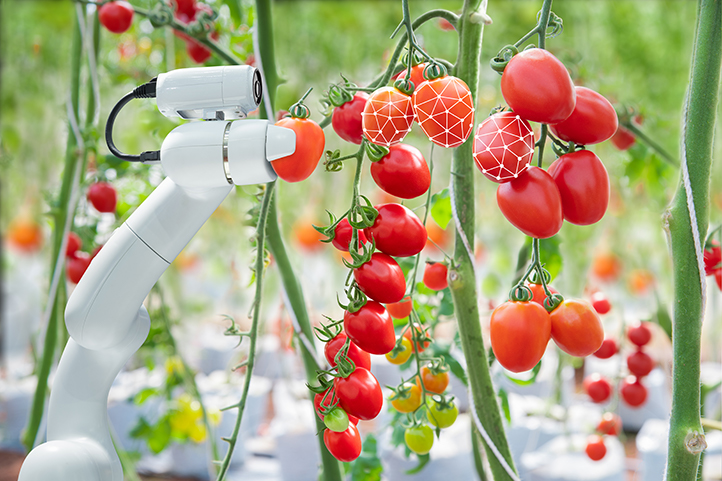
\includegraphics[width=0.8\textwidth]{TomatoPickerBot}
%   \label{fig:tomatoBot}
% \end{figure}
%}
% --- title page setup ---
\USNtitlepage%
%% Please provide the following information:
%% #1 optional figure (set to {} if not wanted)
{%
  {\normalsize}
   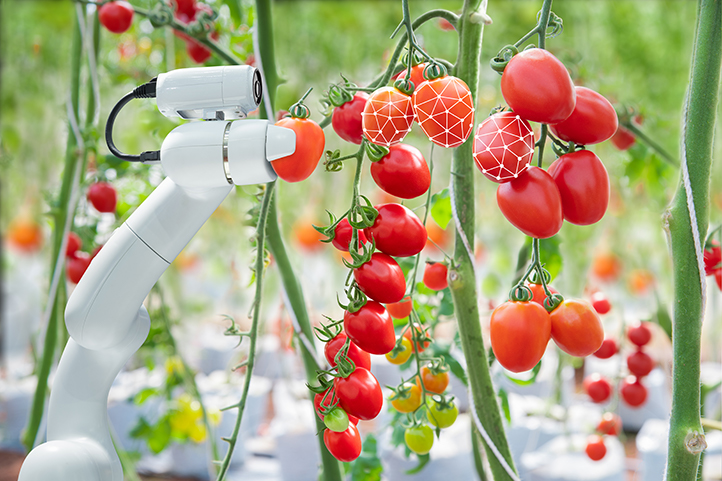
\includegraphics[width=\textwidth]{TomatoPickerBot}}
%% #2 Project partner:
{<Project partner>}
%% #3 Summary:
{%
\lipsum[6-7]
}


%\chapter*{Preface}
%\label{ch:preface}
%\addcontentsline{toc}{chapter}{Preface}
%\lipsum[1-3]
%\bigskip
%Porsgrunn, \today

%\myauthor %% for thesis
%\myparticipants %% for project


%% table of contents
\tableofcontents
\addcontentsline{toc}{chapter}{\contentsname}

%\listoffigures % out-comment if unwanted
%\addcontentsline{toc}{section}{\listfigurename}

%\listoftables  % out-comment if unwanted
%\addcontentsline{toc}{section}{\listtablename}

\chapter{Key drivers and systems architecting}
\label{ch:keyDrivers}
This chapter includes a discussion on key drivers for the fruit-picker robot.
\section{Key drivers}
There are several key drivers or motivations for developing and using the fruit-picker robot. The following are the most apparent:
Quality, environmentally friendly, decreased OpEx, labor independence, efficiency, punctuality, digitalization, ease of expansion, and ease of maintenance.

Customers:
Quality should be closely related to a stakeholder requirement of maintaining the produce quality, it should not be acceptable to damage more berries due to robotic picking. Fruit damage due to picking should be decreased due to robotic precision. Customers want the fruits to be in the best condition possible.
Environmentally friendly, the solution should eliminate the need for foreign workers that produce a lot of emissions due to travel. Understandably, the life cycle assessment for a robot is quite different to a human worker, but should with good practice become a positive decrease over time. The stakeholder requirement will be to keep the emissions as low as possible.

Farmer:
Decreased OpEx, hiring the robot for the fruit-picking job should yield cheaper operational expenditures compared to human labor. The stakeholder requirement has to be to keep the operational costs as low or lower than using foreign labor. If it is more expensive than the old practice, few farmers will be interested. Stakeholder requirement will be to keep operational costs lower than before.
Labor independence, the financial situation might improve further so that cheap foreign workers will become unavailable. Using robots will ensure that tools will be available for harvesting the fruit. The stakeholder requirement will be to keep the ability to harvest in a competitive labor market.
Efficiency, robots can work faster and more energy efficiently than humans. The stakeholder requirement would be that the robot works at least as fast as a human.
Punctuality, picking timings can be improved to meet market behaviors. If there is an event or simply forecasted good weather, the robots can pick fruit in a timely fashion as to meet the expected demand. This will lead to happier costumers in multiple nodes of the value chain. The stakeholder requirement will be to be able to pick fruit with the same or improved time control compared to current methods.
Digitalization, knowledge is power. The robots can track and save all kinds of useful information, such as: when and where ripe fruit is collected. Data scientists can potentially combine this data with e.g. weather data to find useful correlations that can be used to improve yields. The stakeholder requirement will be to gather more and reliable statistics.
Ease of expansion, if the farm is expanding or otherwise needs more robots, it will be easy to configure and calibrate new robots with models developed for the existing robots. The stakeholder requirement is that expansions can be done with a low time investment.
Ease of maintenance, wear and tear is inevitable, by offering a leasing model, a tight connection between robot supplier and costumer (farmer) will include maintenance deals and quick replacements. Meaning it should be possible to replace a robot on short notice and collect the defunct robot for repairing. This could also go into reliability. The stakeholder requirement will be to minimize downtime due to hardware failure.

\chapter{Key drivers and UN goal}
\label{ch:keyDriversUn}

\section{What is a sustainable autonomous system?}
Sustainability is the broad aim for humans to be able to live out their lives on Earth by leaving it in the same or better condition as when they were born \cite{enwiki:1113015553}. Sustainability is made up by the three pillars: environment, economy and society, see figure \ref{fig:whatIsSus}. Sustainable development refers to the path to sustainability and UN has defined 17 development goals in order to reach sustainability. AI and technology, including autonomous systems can both aid and hinder the path towards these goals \cite{vinuesa2020role}. Singular systems can touch upon multiple targets within multiple of the goals and affect them differently. Therefore, a sustainable autonomous system must be a system that greatly favors aiding compared to hindering of the goals and their targets.

\begin{figure}[!ht]
  \centering
  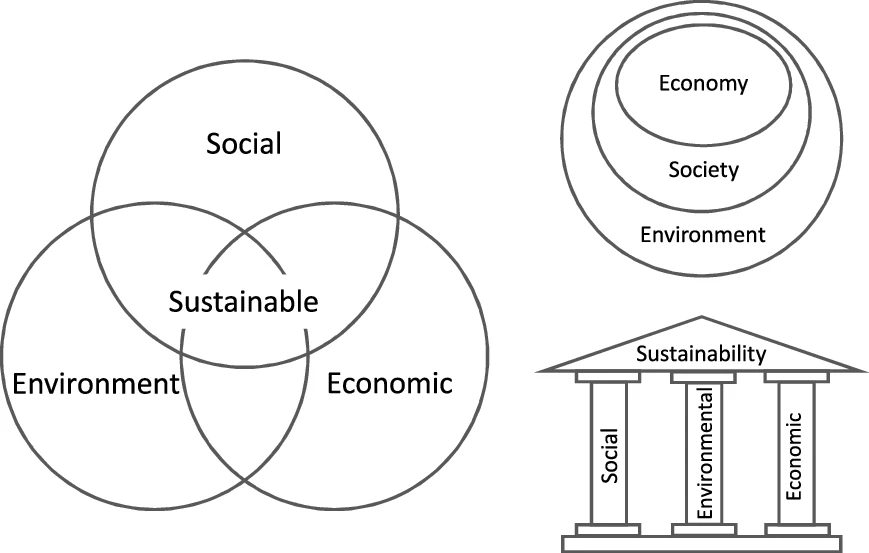
\includegraphics[width=0.8\textwidth]{WhatIsSustainability}
  \caption{Sustainability is the balance between environment, economy and society \cite{enwiki:1113015553}.}
  \label{fig:whatIsSus}
\end{figure}

\section{The fruit-pickers key drivers in relation to UNs SDGs}
Chapter \ref{ch:keyDrivers} shed light on the following key drivers for the berry-picker robot: Quality, environmentally friendly, decreased OpEx, labor independence, efficiency, punctuality, digitalization, ease of expansion, and ease of maintenance.
The UNs sustainability development goals that are related to the berry-picker might just be all of them in a holistic sense. But the following seem most relatable: 1. No poverty, 2. Zero hunger, 9. Industry, innovation and infrastructure; 10. Reduced inequalities, 11. Sustainable cities and communities, 12. Responsible consumption and production, and 13. Climate action.
In comparison, these aren't directed specifically to consumer or owner stakeholders in the same sense as the previous key drivers. Rather they are drivers that affect everybody.

\chapter{Safety and security part I}
\label{ch:safety1}
Safety is related to accidents, unplanned mishaps. Measures can be taken to reduce risk and increase safety. E.g., a worker falling from an unsafe height and damaging themselves, securing them with a safety harness can reduce the risk.
Security is related to keeping something safe or resilient from outside actors. E.g., strongly coded security layers to prevent hacking and theft of the robot.

Potential safety issues:
Berry destruction
Robot damage
Human damage
Animal damage
Plant damage
Fire


Potential security issues:
theft
hacking
vandalism
Animal attacks

\begin{figure}[!ht]
  \centering
  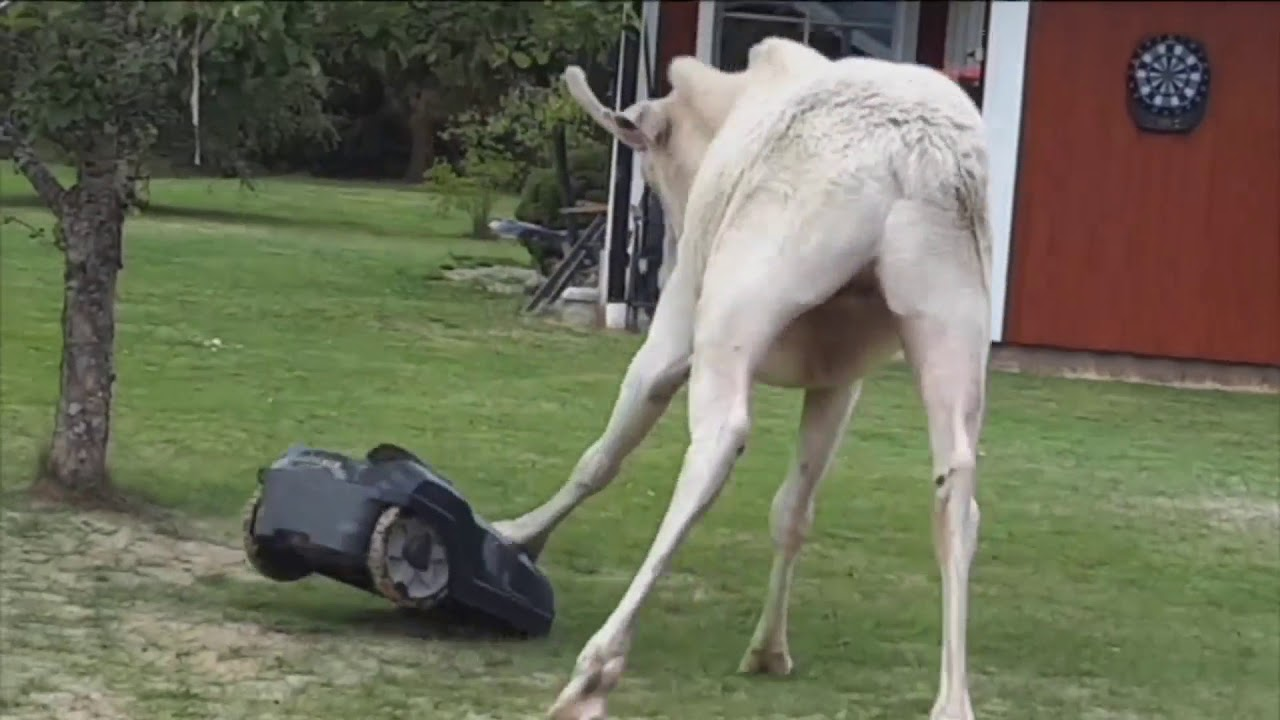
\includegraphics[width=0.8\textwidth]{RobotAttackingMoose}
  \caption{An angry moose unleashed on a robot lawnmower.}
  \label{fig:anAngryMoose}
\end{figure}

\chapter{Safety and security part II}
\label{ch:safety2}

\chapter{Business cases}
\label{ch:Business}


% A dummy command that causes all bibliographyentries to be displayed
% even though there were not cited in the document. Used for demonstration
% purposes only in this template file.
~\nocite{*}

\cleardoublepage

% The bibliography should be displayed here...
%\printbibliography[heading=bibintoc]
% You rather like to call the bibliography "References"? Then use this instead:
%\printbibliography[heading=bibintoc, title={References}]


%\appendix
%\renewcommand{\appendixname}{Paper} %% So we get 'Paper X' displayed instead


%\chapter[Short Title of Paper A]{Title of Paper A (probably very long and therefore not good to have in the header)}
%\label{paper-a}
%
%\paragraph{Note}
%Since some papers tend to have a rather long title it is good to provide the optional short title which then will be displayed in the table of contents and header instead of the long original title.
%On the openening page of the chapter the orginal \emph{long} title will be displayed.\bigskip
%
%\emph{Short descriptive text of paper follows here.}\bigskip
%
%The paper itself needs to be included in the published form as PDF on the next pages.
%This can be done using the \texttt{pdfpages} package by adding the command:
%
%\begin{verbatim}
%\includepdf{pages=-,openright}{Filename}
%\end{verbatim}
%
%You can omit the \texttt{.pdf} when specifying the \texttt{Filename}. Also you should include always include the option \texttt{openright} since it would look strange to have the paper starting at the back of the cover page.
%
%There are more options like only adding specific pages:
%\begin{verbatim}
%\includepdf{pages=2-6,openright}{Filename.pdf}
%\end{verbatim}

%For more options see Appendix~\ref{paper-b} where the most important pages of the \texttt{pdfpages} manual were inlcuded using \texttt{pdfpages}.


%%% Command to include a PDF file directly including all pages:


%\chapter[Short Title of Paper B]{Title of Paper B}
%\label{paper-b}
%Short descriptive text of paper follows here.
%
%Here we included the first five pages of the \texttt{pdfpages} manual itself.
%
%\includepdf[pages=1-5,openright]{fig/pdfpages}
%
\end{document}

%%% Local Variables:
%%% mode: latex
%%% TeX-master: t
%%% End:
